
\begin{Exercise}[label={footfall_analysis}]
A concrete ribbed slab floor spans 9 m and has an average mass of \SI{500}{kg/m^2}. The floor is simply supported on either side and has a natural frequency of vibration of \SI{6.3}{Hz}. 
The floor is to be used for aerobics and other similar rhythmic activities at frequencies ranging from 1.5 to \SI{2.5}{Hz} and with contact ratios $\alpha$ between 0.5 and 1. During these activities the average imposed load will remain below \SI{0.75}{kN/m^2} (before dynamic magnification) and the damping ratio can be taken to be \SI{3}{\%}.

\begin{enumerate}[(a)]
    \item Determine the maximum possible resonant displacement and the resulting peak acceleration and bending moment per unit width.
    \item If the floor has been designed for a service load of \SI{5}{kN/m^2}, determine its suitability for the proposed use.
\end{enumerate}

\begin{center}
\pictures{beamPeople}
\hspace{1em}
\pictures{contactRatio}
\end{center}

\shortAnswer (a) $u_{max} = \SI{1.2}{mm}$, $M_{max} = \SI{20}{kN.m/m}$. (b) The floor is suitable for aerobics.\\
References: \cite{chopra}
\end{Exercise}



\begin{Answer}[ref={footfall_analysis}]
The structure properties per unit width using a sine shape function are
$$
m = \int_{0}^{l}w\psi^2dx = \int_{0}^{l}w\sin^2\left(\frac{\pi x}{l}\right)dx = \frac{wl}{2} = \frac{500\times9}{2} = \SI{2250}{kg/m}
$$
$$
k = \omega^2m = \left(\frac{6.3}{2\pi}\right)^2\times2250 = \SI{9000}{kN/m^2}
$$
and the generalized force is
$$
\tilde{F} = \int_{0}^{l}F\psi dx = \frac{2Fl}{\pi}
$$
The transient walking force considered is a periodic loading with a piecewise definition. Because the action is periodic, a different approach from that of Example \ref{moving_load} can be followed. The action will be approximated using a Fourier series, which is valid for any periodic action.

\paragraph{Pre-computed Fourier terms}

Each component of a Fourier series is also known as a harmonic. For a half sine activity, the amplitudes of the first four harmonics are the following:

\begin{center}
\begin{tabular}{|l|c|cccc|}
    \hline
    Activity & $\alpha$ & $F_1/F_{avg}$ & $F_2/F_{avg}$ & $F_3/F_{avg}$ & $F_4/F_{avg}$ \\ \hline
    Walking  &    2/3   &   1.29   &   0.16   &   0.13   &   0.04   \\
    Exercise &    1/2   &   1.57   &   0.67   &   0.00   &   0.13   \\
    Jumping  &    1/3   &   1.80   &   1.29   &   0.67   &   0.16   \\
    High jumping & 1/4  &   1.89   &   1.57   &   1.13   &   0.67   \\ \hline
\end{tabular}
\end{center}
Then, the dynamic force is the superposition of the static force and the harmonics multiplied by the corresponding dynamic magnification factor:
$$
F_e = F_{avg} + H_1F_1 + H_2F_2 + H_3F_3 + \dots
$$

For the frequency of vibration of \qty{1.5}{Hz}
\begin{align*}
\gamma_1 = \frac{6.3}{1.5} = 4.2\ &\rightarrow\ H_1 = \frac{1}{\sqrt{(1-4.2^2)^2 + 4\times0.03^2\times4.2^2}} = 0.06\\
\gamma_2 = \frac{6.3}{3}   = 2.1\ &\rightarrow\ H_1 = \frac{1}{\sqrt{(1-2.1^2)^2 + 4\times0.03^2\times2.1^2}} = 0.29\\
\gamma_3 = \frac{6.3}{4.5} = 1.4\ &\rightarrow\ H_1 = \frac{1}{\sqrt{(1-1.4^2)^2 + 4\times0.03^2\times1.4^2}} = 1.03\\
\gamma_4 = \frac{6.3}{6}   = 1.05\ &\rightarrow\ H_1 = \frac{1}{\sqrt{(1-1.05^2)^2 + 4\times0.03^2\times1.05^2}} = 8.3\ .
\end{align*}

For walking, the contact ratio $\alpha$ is $2/3$ and the distributed force
$$
F_e = F_{avg} (1 + 0.06\cdot1.29 + 0.29\cdot0.16 + 1.03\cdot0.13 + 8.3\cdot0.04) = 1.59F_{avg}\ .
$$

For exercise, the contact ratio $\alpha$ is $0.5$ and the distributed force
$$
F_e = F_{avg} (1 + 0.06\cdot1.57 + 0.29\cdot0.67 + 8.3\cdot0.13) = 2.37F_{avg}\ .
$$

For the highest frequency of vibration of \qty{2.5}{Hz}
\begin{align*}
\gamma_1 = \frac{6.3}{2.5} = 2.5\ &\rightarrow\ H_1 = \frac{1}{\sqrt{(1-2.5^2)^2 + 4\times0.03^2\times2.5^2}} = 0.19\\
\gamma_2 = \frac{6.3}{5} = 1.26\ &\rightarrow\ H_1 = \frac{1}{\sqrt{(1-1.26^2)^2 + 4\times0.03^2\times1.26^2}} = 1.7\\
\gamma_3 = \frac{6.3}{7.5} = 0.84\ &\rightarrow\ H_1 = \frac{1}{\sqrt{(1-0.84^2)^2 + 4\times0.03^2\times0.84^2}} = 3.4\\
\gamma_4 = \frac{6.3}{10} = 0.63\ &\rightarrow\ H_1 = \frac{1}{\sqrt{(1-0.63^2)^2 + 4\times0.03^2\times0.63^2}} = 1.6\ .
\end{align*}

For walking, the contact ratio $\alpha$ is $2/3$ and the distributed force
$$
F_e = F_{avg} (1 + 0.19\cdot1.29 + 1.7\cdot0.16 + 3.4\cdot0.13 + 1.6\cdot0.04) = 2.02F_{avg}\ .
$$

For exercise, the contact ratio $\alpha$ is $0.5$ and the distributed force
$$
F_e = F_{avg} (1 + 0.19\cdot1.57 + 1.7\cdot0.67 + 1.6\cdot0.13) = 2.65F_{avg}\ .
$$

It can be seen that the higher contact ratio generates a higher dynamic action and that a frequency closer to the structure frequency has a higher dynamic magnification factor. Therefore, we will consider $\alpha=0.5$ and \qty{2.5}{Hz} as the worst scenario.
Finally, the maximum resonant displacement is
$$
u_{max} = \frac{\tilde{F}_e}{k} = \frac{2F_el}{\pi k} = \frac{2\times2.65\times0.75\times9}{9000\pi} = \SI{0.0012}{m} = \SI{1.2}{mm}
$$
and the maximum bending moment per unit width for a uniformly distributed load is
$$
M_{max} = \frac{F_el^2}{8} = \frac{2.65\times0.75\times9^2}{8} = \SI{20}{kN.m/m}
$$


\paragraph{Calculation of the Fourier terms}
Most commonly, Fourier series are expressed as a linear combination of $\sin$ and $\cos$,
$$
F(t) \approx \frac{a_0}{2} + \sum_{n=0}^{\infty} \left(a_n\cos(n\Omega t) + b_n\sin(n\Omega t)\right)
$$
with
\begin{align*}
a_0 &= \frac{2}{T}\int_{0}^{T} F(t) dt \\
a_n &= \frac{2}{T}\int_{0}^{T} F(t) \cos(n\Omega t) dt \\
b_n &= \frac{2}{T}\int_{0}^{T} F(t) \sin(n\Omega t) dt \ .
\end{align*}

An alternative way is to compute the combination of the trigonometric functions as
$$
F(t) \approx F_0 + \sum_{n=0}^{\infty} F_n\sin(n\Omega t + \phi_n)
$$
with
\begin{align*}
&F_0 = \frac{a_0}{2} \\
&F_n = \sqrt{a_n^2 + b_n^2} \\
&\tan\phi_n = \frac{b_n}{a_n} \\
\end{align*}


\begin{center}
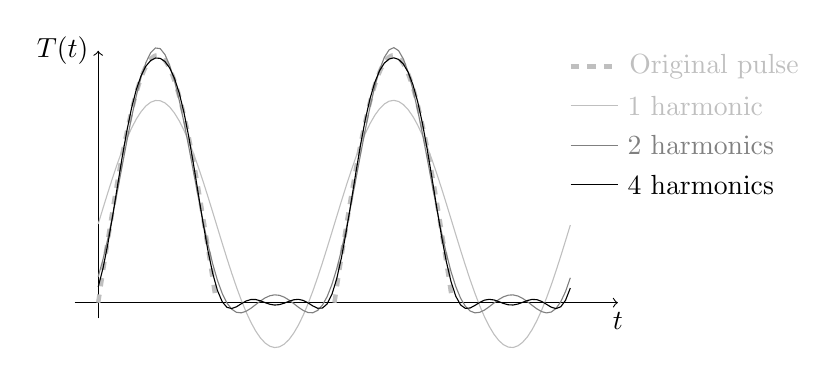
\begin{tikzpicture}[domain=0:2, xscale=3, samples=100]
    \draw[->] (-0.1,0) -- (2.2,0) node[below] {$t$};
    \draw[->] (0,-0.2) -- (0,3.2) node[left] {$T(t)$};

    % \x r means to convert '\x' from degrees to radians:
    \draw[ultra thick,lightgray,dashed,domain=0:0.5] plot (\x,{pi*sin(2*pi*\x r)});
    \draw[ultra thick,lightgray,dashed,domain=1:1.5] plot (\x,{pi*sin(2*pi*\x r)});
    \draw[lightgray] plot (\x,{1+1.57*sin(2*pi*\x r)});
    \draw[gray] plot (\x,{1+1.57*sin(2*pi*\x r)-0.67*cos(4*pi*\x r)});
    \draw[black] plot (\x,{1+1.57*sin(2*pi*\x r)-0.67*cos(4*pi*\x r)-0.13*cos(8*pi*\x r)});

    \draw[ultra thick,lightgray,dashed] (2,3)   -- +(.2,0) node[right] {Original pulse};
    \draw[lightgray]                    (2,2.5) -- +(.2,0) node[right] {1 harmonic};
    \draw[gray]                         (2,2)   -- +(.2,0) node[right] {2 harmonics};
    \draw[black]                        (2,1.5) -- +(.2,0) node[right] {4 harmonics};
\end{tikzpicture}
\end{center}

\end{Answer}
